% Use only LaTeX2e, calling the article.cls class and 12-point type.

\documentclass[12pt]{article}

% Users of the {thebibliography} environment or BibTeX should use the
% scicite.sty package, downloadable from *Science* at
% www.sciencemag.org/about/authors/prep/TeX_help/ .
% This package should properly format in-text
% reference calls and reference-list numbers.

\usepackage{scicite}
\usepackage{amsmath}
\usepackage{soul}

% TO TURN ON/OFF HIGHLIGHTING
 \renewcommand\hl[1]{#1}

\usepackage{array} % for tables
\usepackage{booktabs}
\usepackage[dvipsnames]{xcolor}
\usepackage{geometry} %adjust width
\usepackage{graphicx}%include pdf

% Use times if you have the font installed; otherwise, comment out the
% following line.

\usepackage{times}

% The preamble here sets up a lot of new/revised commands and
% environments.  It's annoying, but please do *not* try to strip these
% out into a separate .sty file (which could lead to the loss of some
% information when we convert the file to other formats).  Instead, keep
% them in the preamble of your main LaTeX source file.


% The following parameters seem to provide a reasonable page setup.

\topmargin 0.0cm
\oddsidemargin 0.2cm
\textwidth 16cm 
\textheight 21cm
\footskip 1.0cm


%The next command sets up an environment for the abstract to your paper.

\newenvironment{sciabstract}{%
\begin{quote} \bf}
{\end{quote}}


% If your reference list includes text notes as well as references,
% include the following line; otherwise, comment it out.

\renewcommand\refname{References and Notes}

% The following lines set up an environment for the last note in the
% reference list, which commonly includes acknowledgments of funding,
% help, etc.  It's intended for users of BibTeX or the {thebibliography}
% environment.  Users who are hand-coding their references at the end
% using a list environment such as {enumerate} can simply add another
% item at the end, and it will be numbered automatically.

\newcounter{lastnote}
\newenvironment{scilastnote}{%
\setcounter{lastnote}{\value{enumiv}}%
\addtocounter{lastnote}{+1}%
\begin{list}%
{\arabic{lastnote}.}
{\setlength{\leftmargin}{.22in}}
{\setlength{\labelsep}{.5em}}}
{\end{list}}


% Include your paper's title here

\title{What incentives can spur Covid-19 vaccination uptake?} 


% Place the author information here.  Please hand-code the contact
% information and notecalls; do *not* use \footnote commands.  Let the
% author contact information appear immediately below the author names
% as shown.  We would also prefer that you don't change the type-size
% settings shown here.

\author
{Heike Klüver,$^{1\ast}$ Felix Hartmann,$^{1}$  Macartan Humphreys,$^{2,3}$\\ Ferdinand Geißler$^{1}$  Johannes Giesecke$^{1}$\\
\\
\normalsize{$^{1}$ Department of Social Science, Humboldt University of Berlin, Germany}\\
\normalsize{$^{2}$ WZB Berlin Social Science Center, Germany}\\
\normalsize{$^{3}$ Columbia University, USA}\\
\\
\normalsize{$^\ast$To whom correspondence should be addressed; E-mail:  heike.kluever@hu-berlin.de.}
}

% Include the date command, but leave its argument blank.

\date{}



%%%%%%%%%%%%%%%%% END OF PREAMBLE %%%%%%%%%%%%%%%%



\begin{document} 

% Double-space the manuscript.

\baselineskip24pt

% Make the title.

\maketitle 

% Word count: 2691

% Place your abstract within the special {sciabstract} environment.

\begin{sciabstract}
Survey evidence suggests that vaccination hesitancy is too high in many countries to achieve herd immunity against Covid-19. In this study, we assess the effectiveness of three strategies to increase vaccine uptake, namely, providing freedoms, financial remuneration, and vaccination at local doctors. We evaluate these strategies   using a factorial survey experiment administered to 20,500 online survey respondents in Germany. Our results suggest that all three strategies can increase vaccination uptake on the order of 5 percentage points (PP) among the undecided. The combined effects could be as high as 13\% for this group. \hl{The returns from different strategies vary across age groups, however, with older cohorts more responsive to local access and younger cohorts most responsive to enhanced freedoms for vaccinated citizens.}
%These effects are precisely estimated, appear to be additive, and vary in effectiveness across age groups. 
\end{sciabstract}



% In setting up this template for *Science* papers, we've used both
% the \section* command and the \paragraph* command for topical
% divisions.  Which you use will of course depend on the type of paper
% you're writing.  Review Articles tend to have displayed headings, for
% which \section* is more appropriate; Research Articles, when they have
% formal topical divisions at all, tend to signal them with bold text
% that runs into the paragraph, for which \paragraph* is the right
% choice.  Either way, use the asterisk (*) modifier, as shown, to
% suppress numbering.

\section*{Introduction}
Vaccination is the most important instrument to sustainably contain the Covid-19 pandemic. In an unprecedented worldwide effort, a number of vaccines have been successfully developed in record time. However, in order to stop the spread of the virus, it is important that sufficient numbers are willing to get vaccinated. While it is estimated that about 60-70\% of the population needs to be vaccinated to stop the pandemic \cite{Aschwanden2020,Randolph2020}, recent survey evidence suggests that this threshold cannot be met in many countries \cite{Lazarus2020,Sallam2021}. The recent decision of many governments to halt the use of the AstraZeneca vaccine because of possible clotting risks has certainly not helped to convince citizens to get vaccinated against Covid-19. Since a consensus has emerged in most countries that compulsory vaccination is not an option due to fundamental civil rights, the question is how to convince citizens to participate in the vaccination programme. Decision-makers around the world therefore currently debate which strategies can be employed in order to increase vaccination uptake. In this study, we contribute to this discussion by evaluating the effectiveness of three different strategies that governments can adopt to increase the vaccination uptake and identifying for which kinds of populations different approaches are more effective. 

While vaccination hesitancy is a major challenge in the fight against the Covid-19 pandemic, there is very little research on this topic. A number of studies shed light on the level of vaccination hesitancy  across countries \cite{Lazarus2020,Loewen2021,Sallam2021}. Previous studies investigating strategies designed to reduce vaccination hesitancy primarily focused on the effect of information campaigns and political messages, \hl{while research on other policy instruments is sparse} \cite{Duquette2020,Rieger2020,Argote2021a}. Early experimental studies were conducted in a purely hypothetical setting before vaccines were available and arrived at mixed results \cite{Duquette2020,Rieger2020}. A recent study conducted after the first vaccines against Covid-19 were approved  has found that basic information about the vaccine and priming social approval benefits can increase vaccination uptake \cite{Argote2021a}. In a follow-up study, it was  furthermore shown that vaccination uptake is higher for Western-produced vaccines, that simple messages about vaccination efficacy can increase the willingness to get vaccinated and that respondents are most responsive to vaccination messages by medical experts \cite{Argote2021b}. However, there is no evidence so far how policy instruments that go beyond information campaigns and framing can reduce vaccination hesitancy. %\textcolor{green}{LS: Make a point that this in most important}

In this study, we address this question and test the effect of three strategies that governments can apply to raise the willingness to get vaccinated against Covid-19, namely, providing freedoms, financial remuneration, and vaccination at local doctors. We identified these strategies based on previous related research and based on the current political debate revolving around the roll-out of the Covid-19 vaccines. Our strategies focus on altering the costs and benefits of vaccination rather than on argumentation, framing, or moral reasoning (as has been studied in previous research \cite{Duquette2020,Rieger2020,Argote2021a,Argote2021b}). 


The first strategy, \emph{granting freedoms}, refers to policies that only reinstall certain liberties to people who are vaccinated while penalizing those without a vaccination. In an effort to increase vaccination uptake, the Israeli government has for instance introduced the so-called ``green passport'' which grants access to social, cultural or sports events to individuals who are immunized \cite{Wilf-Miron2021}. Other countries such as Germany, the United Kingdom and Chile are also debating immunity passports while the European Union is already preparing the launch of a European-wide vaccination passport. The idea of using incentives of this form to encourage vaccination uptake is not new as for instance Australia's ``no jab no pay'' child benefit scheme or vaccination requirements for daycare and school entry in Germany and many US states show. The second strategy, \emph{financial remuneration} refers to providing citizens monetary incentives for vaccination uptake. A large body of research in behavioural and health economics has shown that monetary incentives can be an effective instrument to steer human behaviour \cite{Kamenica2012,Giles2014}. Most recently, it has been shown that even small financial incentives can strongly increase the usage of a Covid-19 contact tracing app \cite{Munzert2021}. Various policy-makers and academics have accordingly proposed the payment of financial rewards for Covid-19 vaccination \cite{Largent2021,Savulescu2021}. The third strategy, \emph{vaccination at local doctors}, rests on two ideas, namely the reduction of transaction costs and increasing trust  \cite{Volpp2021}. A large body of research has demonstrated that transaction costs are a major reason why citizens do not uptake services or vote in elections \cite{Currie2006,Rosenstone1978} while prior research on vaccination hesitancy has shown that trust is a major predictor for vaccination uptake \cite{Yaqub2014}. Allowing local doctors to vaccinate citizens instead of only administering the vaccine roll-out through central vaccination centres can importantly increase trust and reduce transaction costs (e.g. bureaucratic registration systems, inconvenient and distant locations or wait times).





%-------------------------------------------------------------------------
\section*{Study}
To evaluate the effectiveness of these strategies, we designed an experimental study embedded in a nationally representative survey fielded in Germany. We recruited 20,500 respondents over 20 days from 5 March to 25 March 2021 (for more details, see appendix). Among our sample we found that only 67\% of respondents would accept a vaccine if it were available to them (see Fig. 4 in the appendix). This is close to the low bound for herd immunity \cite{Randolph2020}. Among the remainder, 17\% remain undecided and 16\% would refuse to get vaccinated. Germany takes a middle position in vaccine hesitancy across countries---\cite{Lazarus2020} for instance find an average acceptance rate around 72\% across nineteen countries, though with wide variation. As in other countries examined in \cite{Lazarus2020}, institutional trust is an important correlate of hesitancy in Germany (see SI) D. Moreover the primary arguments given for vaccine hesitancy are not specific to the German context: %\textcolor{green}{LS: I think this requires more discussion. How will the results travel? Show Statistics in SI on vaccination campaign + vaccination hesitation to clearly locate case.} 
\hl{When respondents in our sample give an account for their hesitancy, about two thirds describe concerns over the side effects, or long term adverse effects, of the vaccine, with fewer (19\%) discounting the seriousness of Corona.}  These features give some confidence that findings from Germany have implications that extend beyond the case. 

 


%Of those who were undecided or resistant to get vaccinated, 29\% were worried about the long-term consequences of the vaccine, 26\% were concerned about the side effects.

%Vaccine hesitancy in Germany, our data show, reflects political and social divisions more strongly than economic or demographic positions. As seen in Fig.1, younger respondents and women are more likely to be undecided, but these relations are not substantively large. Similarly, education, employment status, and professional position do little to explain hesitancy in Germany. A constellation of measures of general trust, trust in institutions, and support for the populist right AfD political party powerfully explain hesitancy. A majority of the hesitant respondents either support the AfD (20\%) or support no party (37\%). Among those accepting, there is just 3\% support for the AfD and 21\% support no party.  When respondents give an account for their hesitancy, about two thirds describe concerns over the side effects, or long term adverse effects, of the vaccine, with fewer (19\%) discounting the seriousness of Corona.    



We evaluate the effectiveness of three strategies using a factorial survey experiment. In our experiment participants were randomly exposed to vignettes about a hypothetical policy context which varied along three dimensions: freedoms for vaccinated people (yes, no)\footnote{The wording of the vignette is as follows: ``Special regulations (do not) apply to vaccinated people. For example, even when the Corona incidence is high, they can travel again, visit cinemas, restaurants or concerts and are not subject to any contact restrictions.}, financial incentives for vaccination (no, 25 Euros, 50 Euros) and vaccination at local doctors instead of central vaccination centers (yes, no). Subsequently, respondents were questioned about their willingness to get vaccinated under these different policy scenarios. Each respondent received two vignettes successively (see Tab. 1 in the supplementary materials displaying the vignettes). However, respondents did not see that same profile twice. The factorial survey design allows for estimating the effect of these three strategies on the respondents' willingness to get vaccinated against Covid-19 as well as interactions between factors. As the experiment is embedded in a representative population-based survey we are furthermore able to shed light on how effective these strategies are for different subgroups. We use machine learning approaches to systematically assess how the effectiveness of these three strategies varies across population subgroups. Details about the sample, the experimental design and about the statistical analyses can be found in the supplementary materials. All analyses were preregistered at the Center for Open Science (https://doi.org/10.17605/OSF.IO/H8RKB) and institutional review board approval was obtained at Humboldt-Universität zu Berlin.
%-------------------------------------------------------------------------


%-------------------------------------------------------------------------
\section*{Results}


\paragraph*{Main Effects}  
We first report the main treatment effects of the mass vaccination scenario attributes on the probability that respondents take the vaccine pooling across all respondents and across the two scenarios presented to each respondent. Fig. 2 plots the average effects of the policy strategies (see also model 1 in Tab. 3 in the appendix). Each treatment estimate in the figure should be interpreted relative to a control vignette which described a scenario where vaccination would not be possible at local doctors, not lead to more freedoms, or not involve financial payments. The outcome is measured on a 0-1 scale and can be interpreted as a self-report of a respondent's probability of accepting Covid-19 vaccination.

%%%%%%%%%%%%%
\begin{figure}
 \centering
 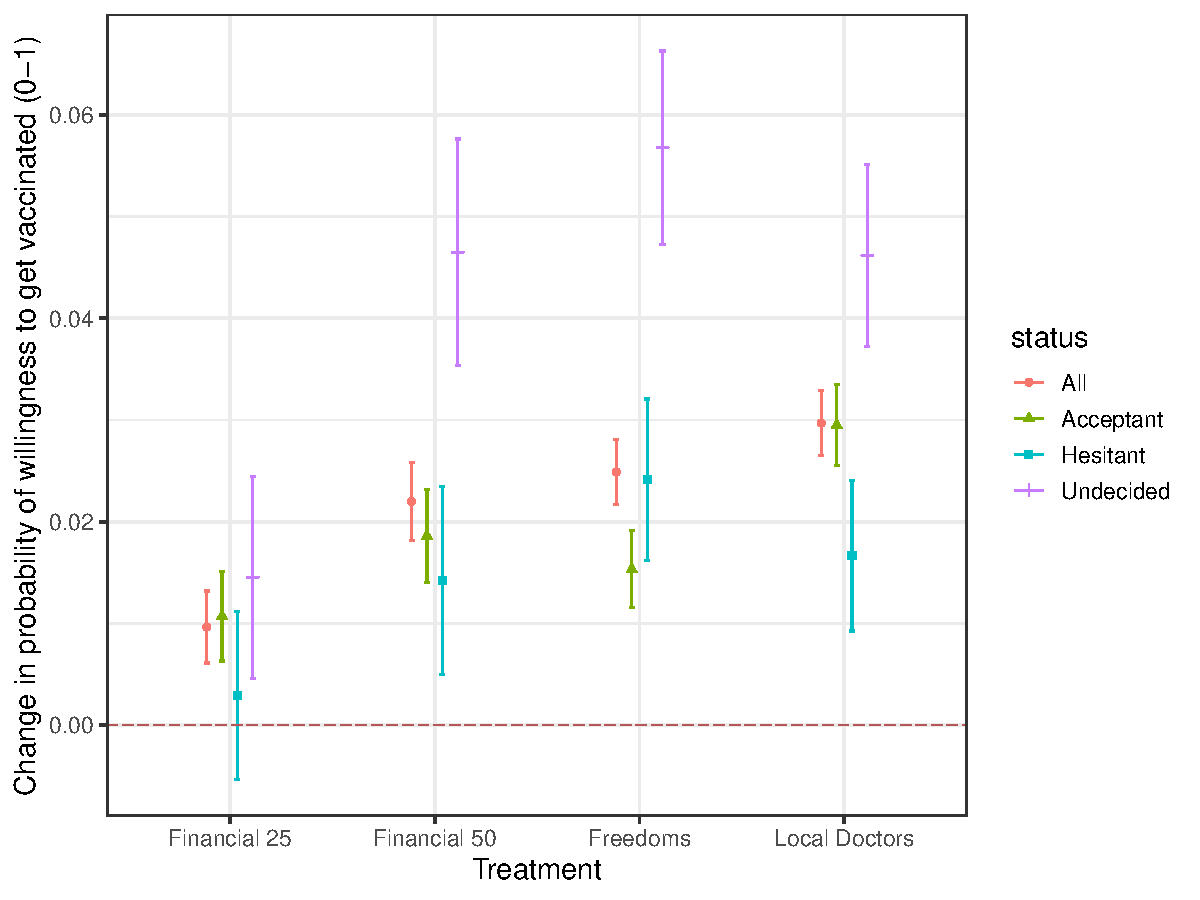
\includegraphics[width=1\linewidth]{figures/figure_2.pdf}
  \caption{\textbf{Effects of mass vaccination scenario attributes on the probability that respondents take the vaccine in the scenario.} Dots with vertical lines indicate point estimates with robust 95\% confidence intervals from linear least squares regression, including individual level fixed effects. Table 3 in the SM displays the underlying regression results.}
\end{figure}

%FG: BITTE DIE Y-ACHSENBESCHRIFTUNG ÄNDERN IN: Change in probability of willingness to get vaccinated (0-1) 

% \textcolor{green}{LS: Is there a beller way to Show overall effect first and in a second fig Conditional on status ?}


%%%%%%%%%%%%%

The results demonstrate that German citizens are responsive to hypothetical changes in the vaccination regime. Three out of four treatments have large and statistically significant effects on the reported willingness to get vaccinated. The size of the average treatment effects of the information vignette varied from 1 to 3 percentage points. We observe the lowest treatment effect for the low financial incentive (25 Euro) with 1 PP,  2.2 PP with high financial incentives (50 Euro), a 2.5 PP increase for the additional freedoms, and a 3 PP increase for vaccinations at the local doctor. All point estimates are significant at a $p < 0.001$. Comparing the effect sizes, we find that doubling the financial incentive corresponds to a more than doubling of an effect on vaccination uptake. Interactions between these treatments are modest and generally not distinguishable from zero.

Next, we investigate if the treatment effects vary by respondents' attitudes towards the vaccination campaign 
\hl{to assess how the effectiveness of these three strategies differs for these subgroups}.  
% MH: seemed repetitive
% which provides insights about which strategies are most effective for which population subgroups}. 
We subset the data for those who accept to get vaccinated, those who remain undecided, and those who are hesitant. While the treatment effects for the acceptants largely correspond to the average effects, we observe large significant differences for hesitant and undecided respondents. Respondents who are hesitant are overall less likely to respond to any treatment conditions. For low financial incentives, we do not observe any significant effect for hesitant respondents and only low effects for the other groups. However, for those who remain undecided, the high financial treatment increases the share of respondents who say that they will get vaccinated by 5 PP ($p < 0.001$). Similarly, the personal freedoms treatment increases the share of respondents who say that they will get vaccinated by 5 PP ($p < 0.001$). We observe the strongest treatment effect (6 PP) among the hesitant for the possibility to get vaccinated at the local doctor. The treatment effect is statistically different from the high financial and freedom treatment at $p < 0.05$. Using an omnibus test we compare the combined treatment effects of all treatments (freedoms incentives, reduced costs, 50 Euro financial incentives) against a combined control group (no freedoms, no reduced costs, no financial incentives). While, among the undecided, the latter group is estimated to have a 40 percent probability of intending to get vaccinated, the corresponding probability of the combined treatment group is estimated to be 13 PP higher ($p < 0.001$) (see Table 4). Given that vaccination acceptance is just a few percentage points below the estimated threshold for herd immunity in many countries \cite{Lazarus2020}, these are sizable effects that could help to achieve community immunity.

% NOTE: CLAIMS IN TEXT ABOUT DIFFERENCES BETWEEN TREATMENT NEED TO BE IN REPLICATION DOCUMENT ALSO

\paragraph*{Heterogenous Effects} We supplement this analysis with a pre-registered machine learning approach \hl{that provides insights about which strategies are most effective for which population subgroups.}   We rely on causal forests \cite{wager2018estimation,athey2016recursive} which is a specific application of the generalized random forests algorithm \cite{athey2019generalized}. We estimate Conditional Average Treatment Effects (CATEs) across all covariates in our data set (details on covariates are given in Appendix C). The approach randomly partitions the data and identifies which regression trees predict the largest variation in the magnitude of treatment effects (for details, see Appendix A). To summarize the results from the causal forests, we calculate a measure of variable 'importance' used to estimate the heterogeneous treatment effects by taking a simple weighted sum of how often a variable was used in a tree split. The results (shown in detail in Fig. 7 in the Appendix) suggest that the age of the respondent, the date of the survey, the level of support for social distancing measure, general solidarity, and vaccination undecidedness are the most important predictors of heterogeneous treatment effects in our sample.


%%%%%%%%%%%%%
% HK: THIS COULD GO INTO THE APPENDIX 
%%%%%%%%%%%%%
%\begin{figure}
% \centering
% 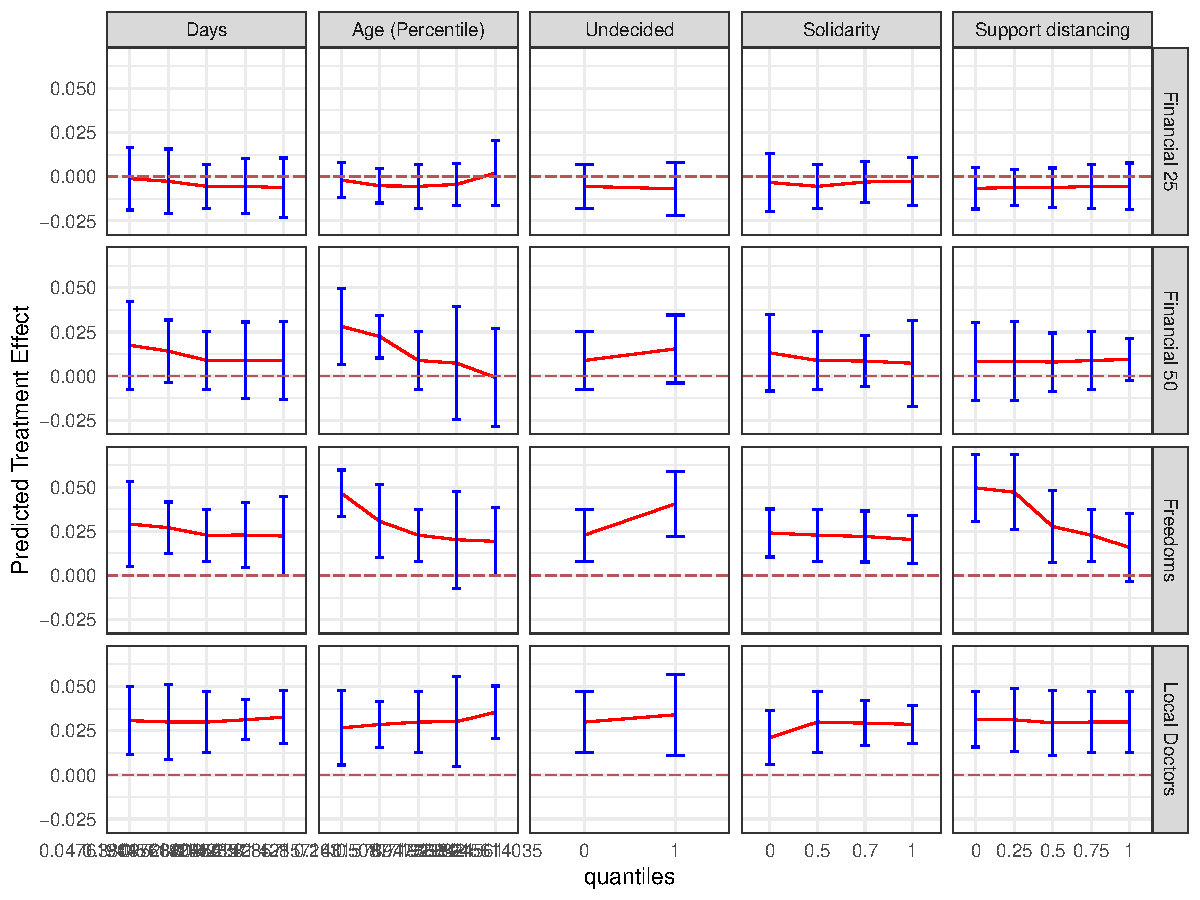
\includegraphics[width=1\linewidth]{figures/figure_4.pdf}
%  \caption{\textbf{Effects of mass vaccination scenario attributes on the probability that respondents take the vaccine in the scenario.} Dots with horizontal lines indicate point estimates with robust 95\% confidence intervals (CI) from predicted causal forests, including individual level fixed effects. }
%\end{figure}

%JG: X-ACHSENBESCHRIFTUNG IRREFÜHREND. SIND KEINE QUANTILE SONDERN EINFACH NUR AUSPRÄGUNGEN DER JEWEILIGEN VARIABLEN
%JG: FERDI UND ICH DENKEN, DASS DIE VARIABLE "UNDECIDED" HIER NICHT HINGEHÖRT (WEIL SIE KEINE KOVARIATE IST). BESSER WÄRE ES SOGAR, DIESE ANALYSE FÜR ALLE ALLE IMPFGRUPPEN ZU MACHEN (ALSO GESAMT, ACCEPTANT, UNDECIDED; HESITANT,) 


\begin{figure}
	\centering
	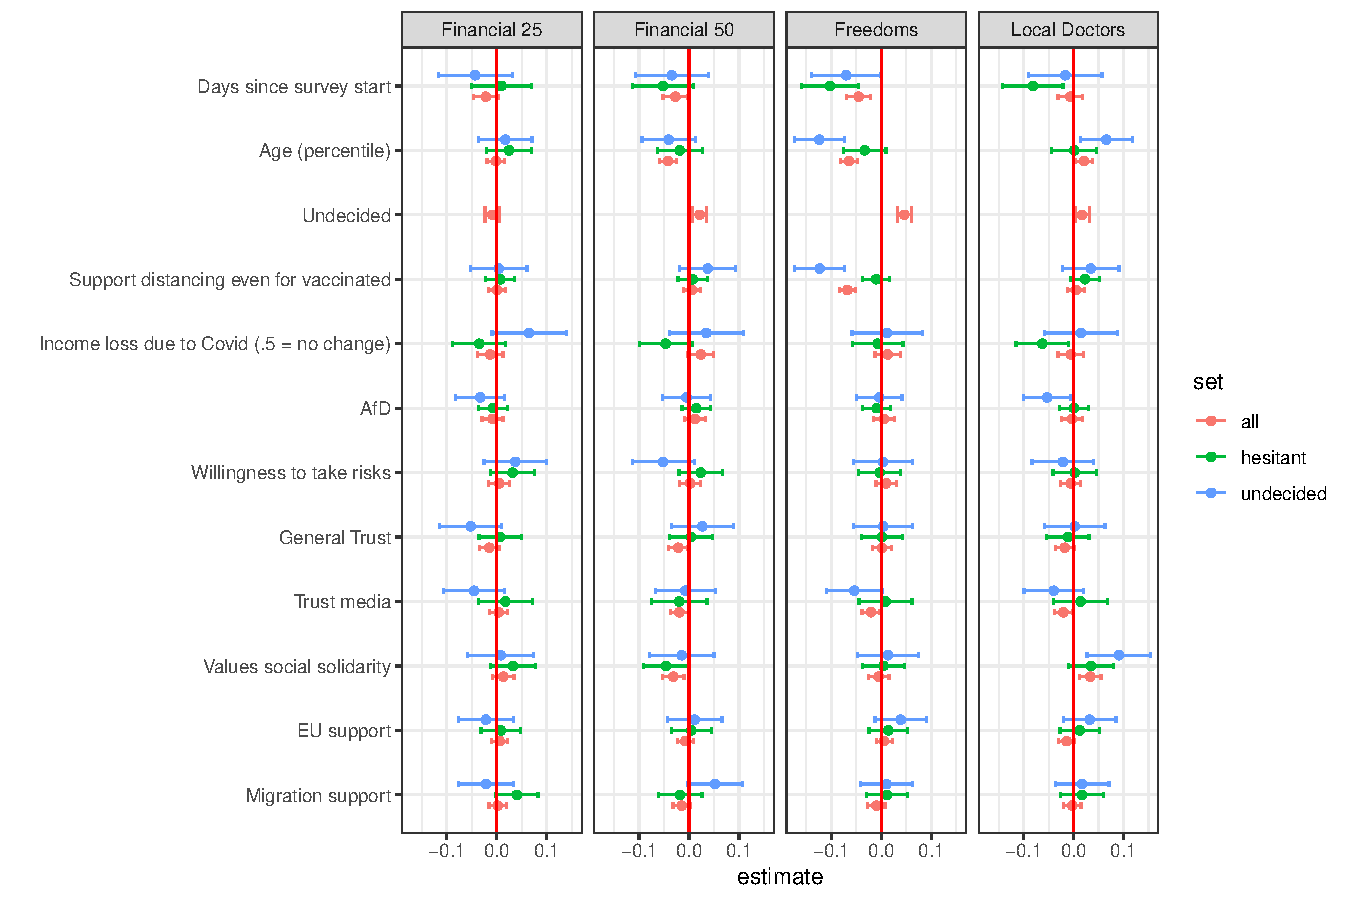
\includegraphics[width=1\linewidth]{figures/figure_9.pdf}
	\caption{\textbf{Features that account for heterogeneity in treatment effects.} Dots indicate the coefficient for the best linear projections of covariates on effect heterogeneity, with positive (resp. negative) numbers indicating that average effects are more positive at higher (resp. lower) values of the covariate. Horizontal lines indicate point estimates with robust 95\% confidence intervals (CI) from predicted causal forests, including individual level fixed effects. }
\end{figure}

%%%%%%%%%%%%%

% HK: This paragraph could be shortened
%Next, we explore how CATE estimates behave when we change a single covariate, while keeping all the other covariates at some fixed value. In Fig. 3 we evaluate a variable of interest across quantiles, while keeping all other covariates at their median. The covariate \textit{Date} refers to the days since the start of the survey implementation (5th of March). We find no predicted heterogeneity for low financial incentives and possibility of vaccination at the local doctor. We do find that high financial incentives and increased personal freedoms predict stronger treatment effect during the earlier periods of the study, but are rendered insignificant during later periods, in particular in case of financial incentives. The lower predicted treatment effects in the later periods could reflect the increased uncertainty about the risk of vaccinations in the German population during that time. On March 15th, 10 days after the start of the survey, the German federal government agency for disease control and prevention (Robert Koch Institute) announced that vaccinations with AstraZeneca would be temporarily suspended. Leading up and following the announcement there has been large public interest in the topic (see Fig. 5 in the appendix). It is precisely during this period (days 8-12 of the survey) where we observe weaker predicted treatment effects. We find a negative interaction effect between the high financial and increased freedoms treatment and the \textit{Age} of the respondents. While both treatment show significant effects for younger cohorts, they are less likely to yield significant effects for older subgroups. The possibility to get vaccinated at the local doctor yields slightly stronger predicted treatment effects for the older cohorts in the study. Using the causal forest, we also find evidence that attitudes towards the vaccination explain heterogeneity in the treatment effects. Those respondents who stated that they were \textit{undecided} to get vaccinated showed higher treatment effects for high financial incentives and personal freedoms. Further, increased personal freedoms are predicted to yield higher CATE's for those who show less \textit{solidarity} with others in the society (low values on the scale). The possibility to get vaccinated at the local doctor is more likely to yield treatment effects for those who show more solidarity with others. Lastly, we show that those who do not \textit{support social distancing} once they are vaccinated are also more likely to show strong treatment effects for increased personal freedoms. 


\hl{To see for which population subgroups the strategies have the strongest effect,  Fig. 3 reports coefficients derived from regressing scores based on the causal forest on selected covariates. The most important substantive finding is that the effectiveness of the strategies varies by age groups. While older cohorts are more responsive to the opportunity to get vaccinated at local doctors, younger cohorts are most receptive to granting freedoms to vaccinated citizens. This heterogeneity is illustrated in Fig. 8 in the appendix. In addition we find that respondents who stated that they were \textit{undecided} to get vaccinated showed higher treatment effects for high financial incentives and personal freedoms.  We see suggestive evidence that all four treatments are becoming less effective over time, possibly reflecting a pattern where citizens become more settled in their positions.}



%Finally we point to a small set of moderators that relate to the social divisions in German society we pointed to above. We note first that we do not see marked heterogeneity by partisanship (comparing AfD supporters to others) or broad position on a Left/Right ideology scale. Nor do we see that reactions to treatments depend on the measured trustingness of respondents. We do see however that hesitant respondents that report more solidarity, are generally more responsive to Local Doctors (and less responsive to financial incentives). Overall these treatments do little to alter the pattern of differences between hesitant and acceptant respondents. 

%-------------------------------------------------------------------------
\section*{Conclusion}
%This study examined the effectiveness of three different policy instruments, namely providing freedoms, financial remuneration and vaccination at local doctors on vaccination uptake against Covid-19. We conducted a large-scale factorial experiment embedded in a representative public opinion survey to evaluate the effectiveness of these strategies among 20,500 German citizens. Our results show that all three strategies can significantly increase vaccination uptake, but that their effect varies across age groups.

Our study assesses citizen responses to three hypothetical policy instruments, namely providing freedoms, financial remuneration, and the possibility of vaccination at local doctors. Our results suggest, first, that governments can increase the willingness to get vaccinated if they distribute vaccines through the established  network of local doctors. Governments can increase vaccination uptake by exploiting the trustful relationships between citizens and their local doctors and avoiding bureaucratic hassle and long wait and travel times that typically come with central vaccination centers. In addition, granting vaccinated people rights that are not available to non-vaccinated citizens can encourage uptake among the undecided, for instance by restricting participation in larger social events to vaccinated citizens. Financial rewards can also be an instrument to increase vaccination uptake, but our results suggests payments have to be sizable. These strategies can be combined and largely appear not to substitute for each other. 

\hl{Different approaches vary in their effectiveness for different segments of the population however. While all three strategies have positive average effects on reported acceptance,  our findings suggest that the scope for altering behavior among truly hesitant respondents is limited. Governments can do better by focusing on undecided citizens for which the combined effects for all three strategies could be as high as 13\%. In addition, the choice of strategy depends on the age profile of undecided citizens, in particular governments seeking to increase vaccination uptake among undecided younger cohorts may see greater returns from enhancing freedoms while governments focused on undecided older citizens will see greater returns from ensuring provision at local doctors.} 






% MH: Need to add caveats: it's justa survey. 
% Need to compare to results from other treatments; perhaps speculate on impact of AfD leadership taking a position

%In addition to these main results, our study assesses for which respondents different treatments are more or less effective. Broadly we find that heterogeneity in effects is not very strong %and does not relate strongly to the correlates of hesitancy, such as indicators of trust or AfD party support. 
%However there is relatively consistent evidence for differential responsiveness across age groups with vaccination at local doctors most effective for increasing vaccination uptake among older undecided respondents while providing freedoms has the largest effect among younger cohorts.


%JG: ES WÄRE NOCH ZU ÜBERLEGEN, DASS HIER NOCH AUF DIE SUBGROUPS (UNDECIDED ETC.) EINGEGANGEN WIRD. DAS IST NÄMLICH SEHR INTERESSANT UND EVENTUELL WÜRDE DIE SUBANALYSE BEI FIG. 3 JA AUCH NOCH WEITERE INTERESSANTE ERGEBNISSE LIEFERN. IST ABER WOHL KEIN PLATZ MEHR... 


%\section*{What to Send In}If you're sending in the initial submission of your manuscript (that is, the copy for evaluation and peer review), please send in {\it only\/} a PostScript or PDF version of the compiled file (including figures).

% Your references go at the end of the main text, and before the
% figures.  For this document we've used BibTeX, the .bib file
% scibib.bib, and the .bst file Science.bst.  The package scicite.sty
% was included to format the reference numbers according to *Science*
% style.

\newpage 

\bibliography{scibib}

\bibliographystyle{Science}



% Following is a new environment, {scilastnote}, that's defined in the
% preamble and that allows authors to add a reference at the end of the
% list that's not signaled in the text; such references are used in
% *Science* for acknowledgments of funding, help, etc.

%\begin{scilastnote}
%\item   Acknowledgements
%\end{scilastnote}




% For your review copy (i.e., the file you initially send in for
% evaluation), you can use the {figure} environment and the
% \includegraphics command to stream your figures into the text, placing
% all figures at the end.  For the final, revised manuscript for
% acceptance and production, however, PostScript or other graphics
% should not be streamed into your compliled file.  Instead, set
% captions as simple paragraphs (with a \noindent tag), setting them
% off from the rest of the text with a \clearpage as shown  below, and
% submit figures as separate files according to the Art Department's
% instructions.


\clearpage
%%%%%%%%%%%%%%%%%%%%%%%%%%%%%%%%%%%%%%%%%%%%%%%%%%%%%%% 


\appendix{\textbf{\Large{A Supplementary Materials}}}
%%%%%%%%%%%%%%%%%%%%%%%%%%%%%%%%%%%%%%%
\tableofcontents


\clearpage
\section{Sample \& Recruitment}  

Our population of interest consists of all German citizens aged 18 to 75 years. We rely on a representative sample of 20,500 citizens across Germany. In order to conduct the factorial survey experiment, we fielded the experiment relying on the online access panel of the survey company Respondi. Respondi relies on online channels and offline channels to recruit new panelists for its online panel. After completing a profiling questionnaire covering basic sociodemographic information, panelists are then invited to participate in surveys. Respondi compensates its panelists for completing a survey. In our study, the incentive was EUR 0.75 for a median length of interview (LOI) of approximately 15 minutes.


\clearpage
\section{Experimental Design}
In the factorial survey experiment, participants were randomly exposed to different hypothetical policy instruments (special rights for vaccinated people, financial incentives for vaccination and vacci-nation at local medical practices) and we subsequently questioned respondents about their willingness to get vaccinated under these different policy scenarios. The experiment relies on a single profile forced choice conjoint experiment using 2x2x3 factorial design, with factors assigned with independent probabilities. Each respondent was asked to indicate the willingness to get vaccinated under two hypothetical policy contexts, and for each profile we randomly assigned the values of all attributes. 
The treatment consists of a vignette consisting of the following policy factors M with randomly assigned levels L.



\newpage
%%%%%%%%%%%%%%%%%%%%%%%%%%
\begin{table}
\centering
\caption{Factors of mass vaccination scenario, by dimension.}
\begin{tabular}[t]{l>{\raggedright}p{0.3\linewidth}>{\raggedright\arraybackslash}p{0.3\linewidth}}
\toprule
Factor $Z$  &Control (0) &Treatment (1) \\
\midrule
Freedoms &There are \textbf{no special regulations} for vaccinated people even when the Corona incidence is high. For example, they cannot travel again, visit cinemas, restaurants or concerts and are still subject to contact restrictions.&\textbf{Special regulations} apply to vaccinated people. For example, even when the Corona incidence is high, they can travel again, visit cinemas, restaurants or concerts and are not subject to any contact restrictions.\\\\
Reduction Transaction Cost& Eligible citizens can get vaccinated against Corona at the nearest vaccination center \textbf{but not at their family doctor}.&Eligible citizens get vaccinated against Corona at the nearest vaccination center \textbf{or at their family doctor}.\\\\
Financial Incentives&Citizens who are vaccinated \textbf{will not receive any allowance} after receiving the vaccination.
&Citizens who get vaccinated \textbf{receive an expense allowance of 25 Euros} after receiving the vaccination.\\
& 
&Citizens who get vaccinated \textbf{receive an expense allowance of 50 Euros} after receiving the vaccination.\\
\bottomrule
\end{tabular}
\end{table}%
%%%%%%%%%%%%%%%%%%%%%%%%%%


Our main outcome variable is the vaccination probability which takes on values between 0 and 10. We rescale the outcome to take on value between 0 and 1. 


\begin{itemize}
\item
  \textbf{Outcome: Vaccination Probability} Please use this scale to indicate how
  likely it is that you would be vaccinated against corona under these
  conditions.

  \begin{itemize}
  \item
    0 I will definitely not be vaccinated against corona
  \item
    1
  \item
    2
  \item
    3
  \item
    4
  \item
    5
  \item
    6
  \item
    7
  \item
    8
  \item
    9
  \item
    10 I am sure to get vaccinated against corona
  \end{itemize}
\end{itemize}


\noindent \textbf{Main Estimation.} We seek to estimate the average effect of each treatment, averaged over other treatment conditions. 
We estimate treatment effects using an OLS regression with individual level fixed effects and heteroskedasticity-robust standard errors:

\begin{eqnarray*}
Y_{it}&=&\beta_0 + \beta_1 Z^1_{it} + \beta_2 Z^2_{it} + \beta_3 Z^\text{3, low}_{it}  + \beta_4 Z^\text{3, high}_{it} + \\
&& \beta_5 Z^1_{it}Z^2_{it} + \beta_6 Z^1_{it}Z^\text{3, low}_{it}  + \beta_7 Z^1_{it}Z^\text{3, high}_{it} + \beta_8 Z^2_{it}Z^\text{3, low}_{it}  + \beta_9 Z^2_{it}Z^\text{3, high}_{it}\\
&&  + \beta_{10} Z^1_{it}Z^2_{it}Z^\text{3, low}_{it} + \beta_{11} Z^1_{it}Z^2_{it}Z^\text{3, low}_{it} + u_i +  \epsilon_{it}
\end{eqnarray*}

where \(Y\) is a continuous variable measuring the reported likelihood of
vaccination of participant \(i\) for two policies ($t\in\{1,2\}$) each described by three conditions $Z^1$ (Freedoms), $Z^2$ (Local Doctor), $Z^{3, low}$ (Financial remuneration 25 Euros), $Z^{3, high}$ (Financial remuneration 50 Euros)). Conditions are centered with 0 mean. With this normalization $\beta_1 - \beta_4$ capture the average fixed effects averaged over conditions of other variables \cite{lin2013agnostic}. 


\clearpage
\section{Descriptive Statistics}  

%%%%%%%%%%%%%%%%%

\begin{table}

\caption{\label{tab:SummStats}Summary statistics}
\centering
\resizebox{\linewidth}{!}{
\begin{tabular}[t]{lrrrrrrr}
\toprule
Variable & Mean & Stdev & Minimum & Lower quartile & Median & Upper quartile & Maximum\\
\midrule
Days since survey start & 0.57 & 0.19 & 0.05 & 0.38 & 0.57 & 0.71 & 1.00\\
Male respondent & 0.50 & 0.50 & 0.00 & 0.00 & 0.00 & 1.00 & 1.00\\
Age (percentile) & 0.49 & 0.27 & 0.00 & 0.26 & 0.51 & 0.72 & 1.00\\
Non German Citizen & 0.03 & 0.16 & 0.00 & 0.00 & 0.00 & 0.00 & 1.00\\
Born outside of Germany & 0.06 & 0.24 & 0.00 & 0.00 & 0.00 & 0.00 & 1.00\\
Migration background of parents & 0.23 & 0.42 & 0.00 & 0.00 & 0.00 & 0.00 & 1.00\\
In former East Germany & 0.15 & 0.36 & 0.00 & 0.00 & 0.00 & 0.00 & 1.00\\
Household size 3 or more & 0.33 & 0.47 & 0.00 & 0.00 & 0.00 & 1.00 & 1.00\\
Employed & 0.44 & 0.50 & 0.00 & 0.00 & 0.00 & 1.00 & 1.00\\
Years of Education & 0.36 & 0.13 & 0.00 & 0.28 & 0.28 & 0.44 & 0.56\\
Previously had Covid & 0.03 & 0.17 & 0.00 & 0.00 & 0.00 & 0.00 & 1.00\\
Members of network infected & 0.40 & 0.36 & 0.00 & 0.00 & 0.50 & 0.50 & 1.00\\
Good general health & 0.65 & 0.23 & 0.00 & 0.50 & 0.67 & 0.83 & 1.00\\
Covid pre-existing conditions & 0.41 & 0.49 & 0.00 & 0.00 & 0.00 & 1.00 & 1.00\\
Share of network vaccinated & 0.25 & 0.24 & 0.00 & 0.00 & 0.25 & 0.50 & 1.00\\
Respondent has been vaccinated & 0.06 & 0.25 & 0.00 & 0.00 & 0.00 & 0.00 & 1.00\\
Refusals & 0.16 & 0.37 & 0.00 & 0.00 & 0.00 & 0.00 & 1.00\\
Undecided & 0.17 & 0.38 & 0.00 & 0.00 & 0.00 & 0.00 & 1.00\\
Acceptant & 0.67 & 0.47 & 0.00 & 0.00 & 1.00 & 1.00 & 1.00\\
Seeks Covid information & 0.73 & 0.32 & 0.00 & 0.50 & 0.75 & 1.00 & 1.00\\
Believes media exaggerates risk & 0.42 & 0.32 & 0.00 & 0.25 & 0.50 & 0.75 & 1.00\\
Compliance: mask rules & 0.90 & 0.16 & 0.00 & 0.80 & 1.00 & 1.00 & 1.00\\
Compliance: distance rule & 0.82 & 0.19 & 0.00 & 0.80 & 0.80 & 1.00 & 1.00\\
Support distancing even for vaccinated & 0.71 & 0.30 & 0.00 & 0.50 & 0.75 & 1.00 & 1.00\\
Income loss due to Covid (.5 = no change) & 0.59 & 0.19 & 0.00 & 0.50 & 0.50 & 0.75 & 1.00\\
Political interest & 0.65 & 0.29 & 0.00 & 0.33 & 0.67 & 1.00 & 1.00\\
Voted last elections & 0.83 & 0.38 & 0.00 & 1.00 & 1.00 & 1.00 & 1.00\\
Right leaning & 0.44 & 0.18 & 0.00 & 0.30 & 0.50 & 0.50 & 1.00\\
AfD & 0.07 & 0.26 & 0.00 & 0.00 & 0.00 & 0.00 & 1.00\\
Conservatives & 0.20 & 0.40 & 0.00 & 0.00 & 0.00 & 0.00 & 1.00\\
Liberals & 0.05 & 0.23 & 0.00 & 0.00 & 0.00 & 0.00 & 1.00\\
Green Party & 0.16 & 0.37 & 0.00 & 0.00 & 0.00 & 0.00 & 1.00\\
Left Party & 0.08 & 0.26 & 0.00 & 0.00 & 0.00 & 0.00 & 1.00\\
Social Democrats & 0.14 & 0.34 & 0.00 & 0.00 & 0.00 & 0.00 & 1.00\\
No party identification & 0.27 & 0.44 & 0.00 & 0.00 & 0.00 & 1.00 & 1.00\\
Willingness to take risks & 0.41 & 0.24 & 0.00 & 0.20 & 0.40 & 0.60 & 1.00\\
General Trust & 0.41 & 0.25 & 0.00 & 0.20 & 0.40 & 0.60 & 1.00\\
Trust state government & 0.44 & 0.29 & 0.00 & 0.25 & 0.50 & 0.75 & 1.00\\
Trust experts & 0.64 & 0.26 & 0.00 & 0.50 & 0.75 & 0.75 & 1.00\\
Trust federal government & 0.45 & 0.27 & 0.00 & 0.25 & 0.50 & 0.75 & 1.00\\
Trust media & 0.38 & 0.25 & 0.00 & 0.25 & 0.50 & 0.50 & 1.00\\
Trust healthcare & 0.57 & 0.26 & 0.00 & 0.50 & 0.50 & 0.75 & 1.00\\
Values social solidarity & 0.58 & 0.23 & 0.00 & 0.50 & 0.50 & 0.70 & 1.00\\
Values international solidarity & 0.58 & 0.31 & 0.00 & 0.40 & 0.50 & 0.80 & 1.00\\
EU support & 0.52 & 0.29 & 0.00 & 0.30 & 0.50 & 0.70 & 1.00\\
Migration support & 0.48 & 0.27 & 0.00 & 0.30 & 0.50 & 0.70 & 1.00\\
Distance to Vaccination Center & 0.13 & 0.10 & 0.00 & 0.06 & 0.11 & 0.18 & 1.00\\
\bottomrule
\end{tabular}}
\end{table}


%%%%%%%%%%%%%%%%%%%%%%%%%%%%%%%%%%% 
%%%%%%%%%%%%%%%%%%%%%%%%%%%%%%%%%%% 
%%%%%%%%%%%%%%%%%%%%%%%%%%%%%%%%%%% 
\begin{figure}[h!]
 \centering
 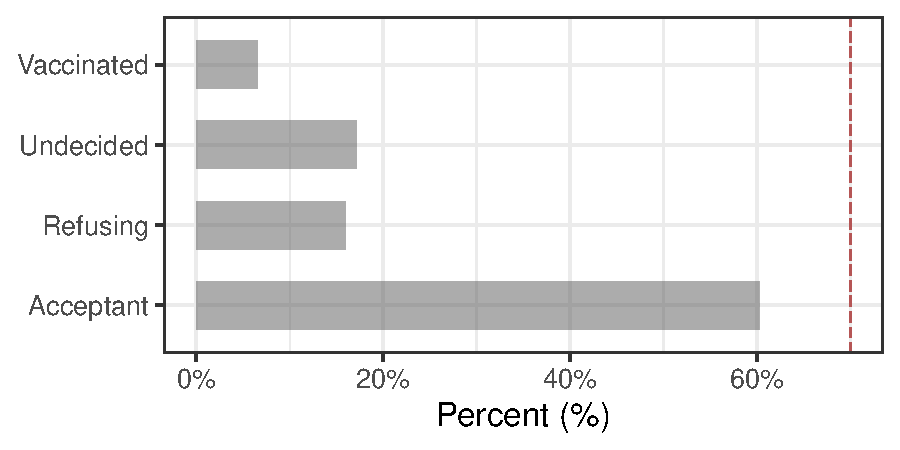
\includegraphics[width=0.8\linewidth]{figures/figure_1.pdf}
 \label{fig:outcomes}
 \caption{Distribution of the outcome variable. Question: Vaccination Probability: Please use this scale to indicate how likely it is that you would be vaccinated against corona under these conditions.}
 \end{figure}
%%%%%%%%%%%%%%%%%%%%%%%%%%%%%%%%%%% 
%%%%%%%%%%%%%%%%%%%%%%%%%%%%%%%%%%% 
\begin{figure}[h!]
 \centering
 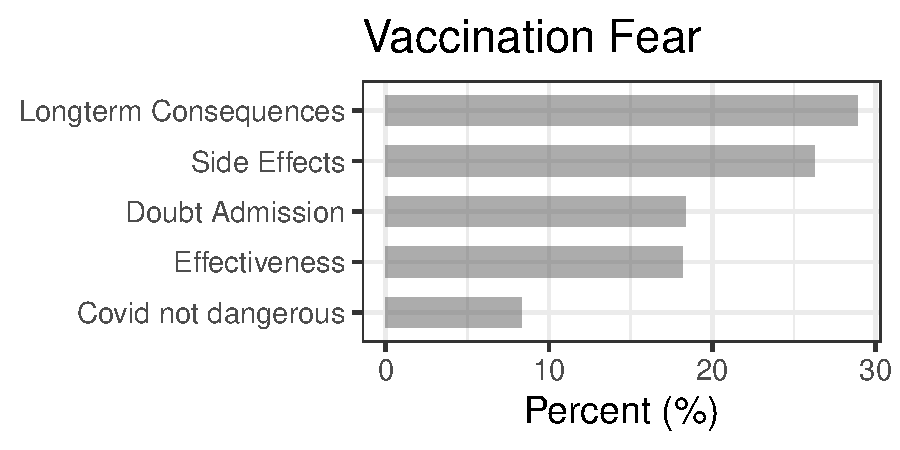
\includegraphics[width=0.8\linewidth]{figures/figure_11.pdf}
 \label{fig:outcomes}
 \caption{Reasons given for being hesitant or undecided.}
 \end{figure}
%%%%%%%%%%%%%%%%%%%%%%%%%%%%%%%%%%% 

\clearpage
\section{Correlates of vaccine hesitancy}
Vaccine hesitancy in Germany, our data show, strongly reflects political and social divisions. As seen in Fig.1, younger respondents and women are more likely to be undecided, but these relations are not substantively large. Similarly employment status, and professional position do little to explain hesitancy in Germany, though education is strongly (negatively) correlated with hesitancy. A constellation of measures of general trust, trust in institutions, and support for the populist right AfD political party powerfully explain hesitancy. A majority of the hesitant respondents either support the AfD (20\%) or support no party (37\%). Among those accepting, there is just 3\% support for the AfD and 21\% support no party. 


% \textcolor{green}{LS: Too much info. Fig could improve too show main take away. Maybe only show hesitant in main text? What are the baselines ? What are the tobust se. for?}

\begin{figure}[h!]
	\centering
	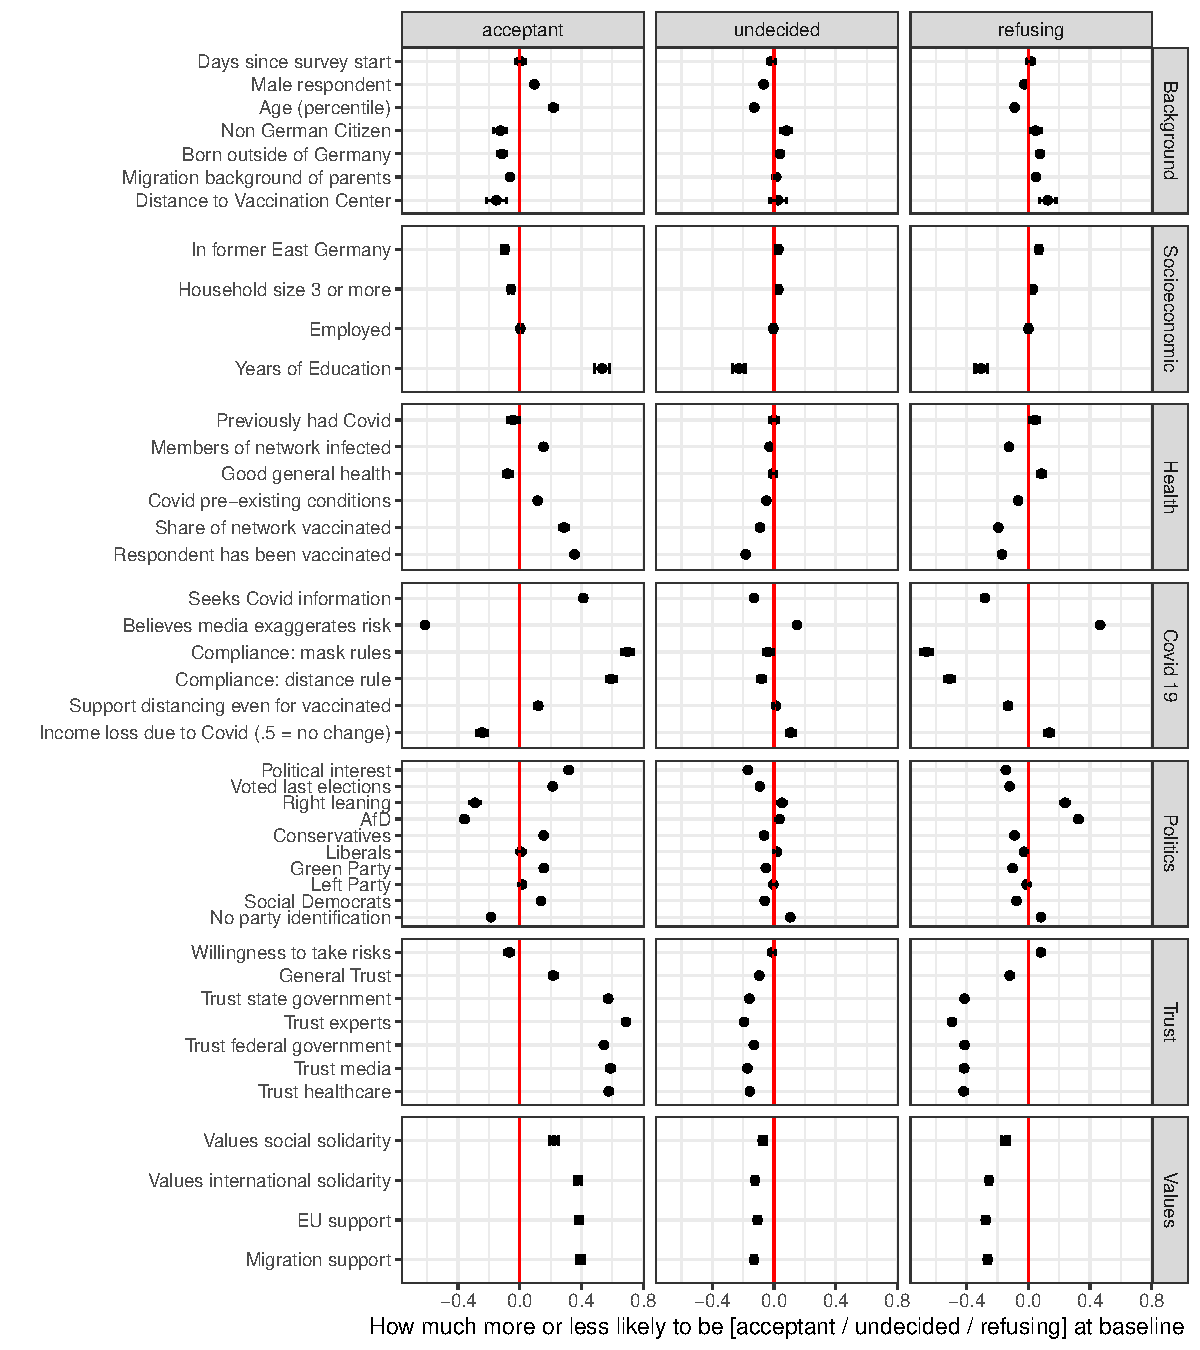
\includegraphics[width=1\linewidth]{figures/figure_7.pdf}
	\caption{\textbf{Correlates of hesitancy.} Coefficient from linear models separately regressing vaccine attitudes (columns) on different covariates with confidence intervals calculated using robust standard errors. Variables range from 0 - 1. }
	\label{correlates}
\end{figure}



\clearpage

\subsection{Correlations between covariates}

%%%%%%%%%%%%%
\begin{figure}[h!]
	\centering
	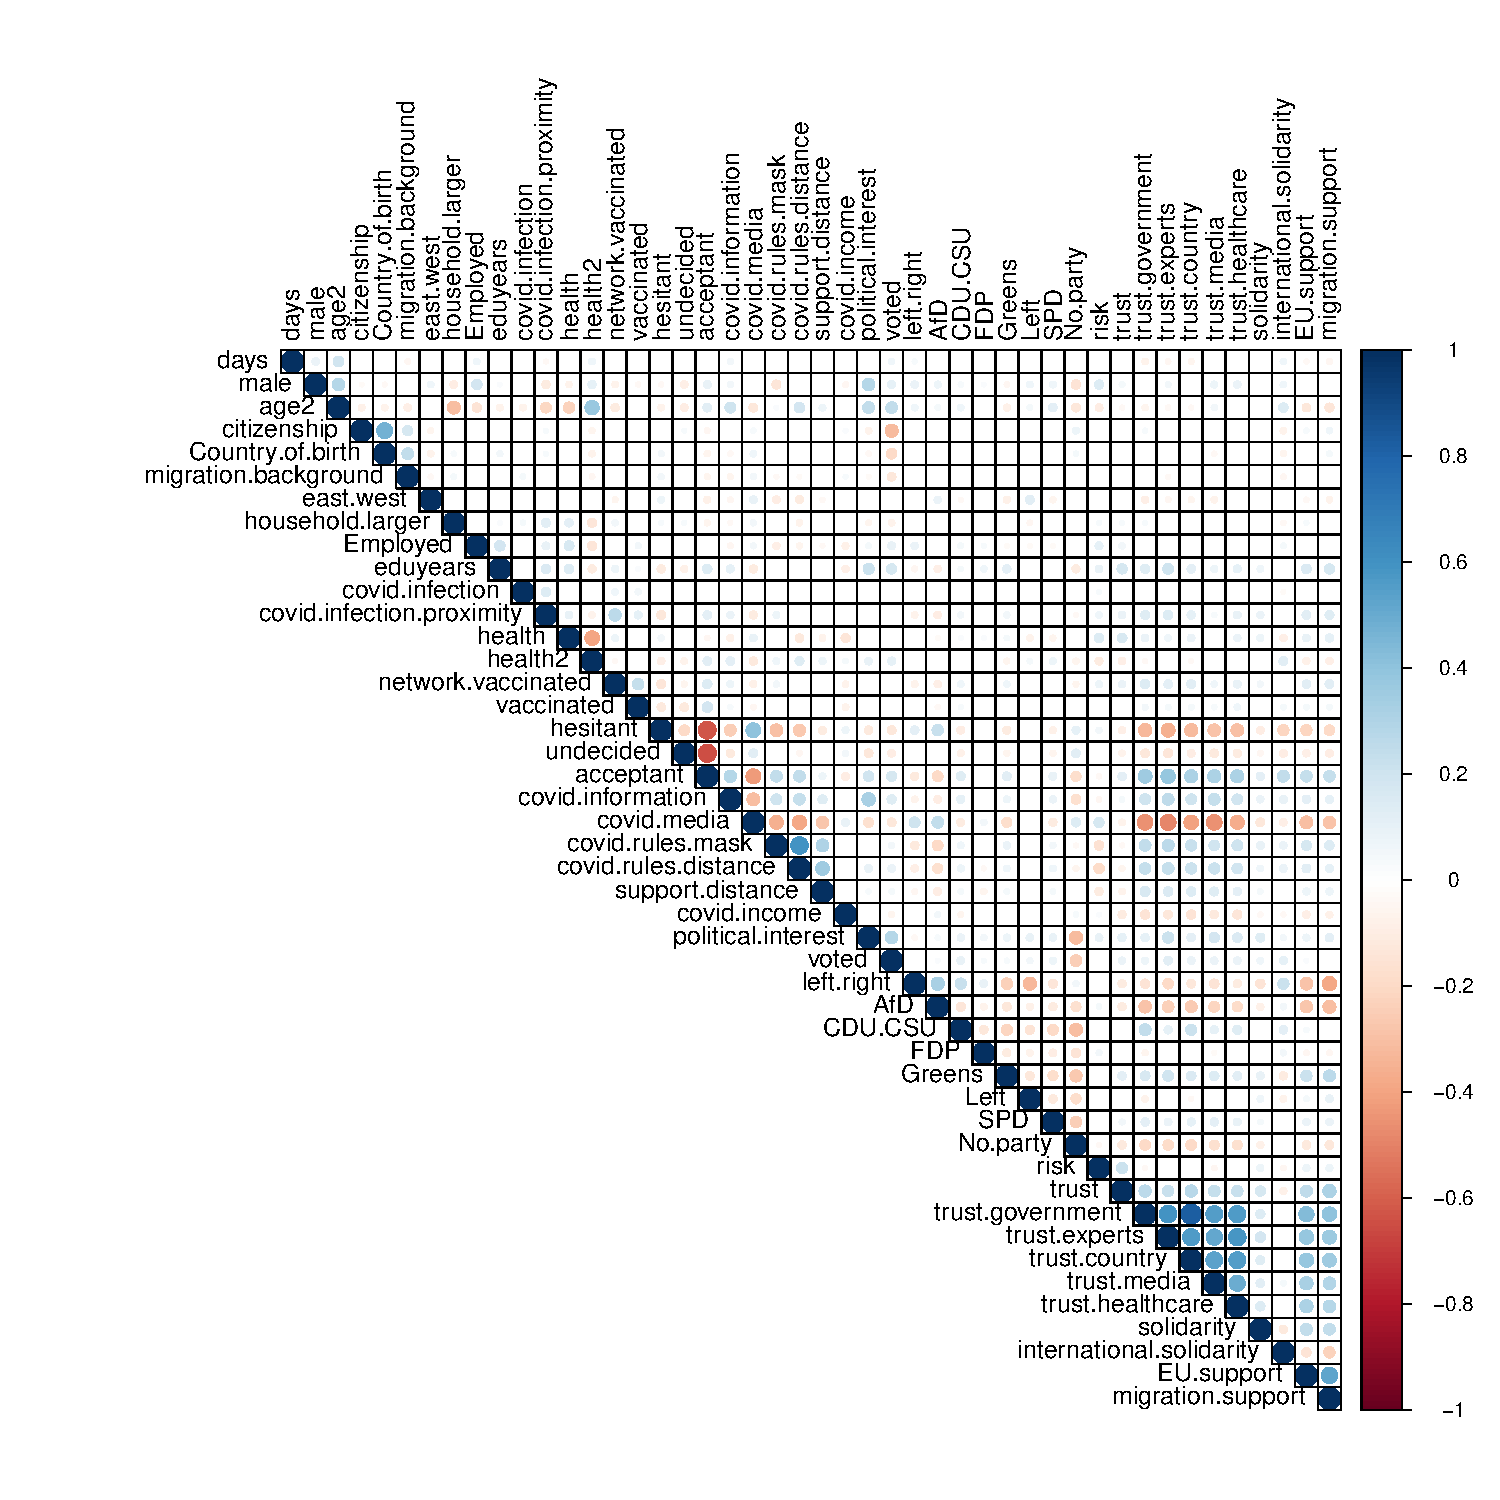
\includegraphics[width=1\linewidth]{figures/figure_6.pdf}
	\caption{A square is colored only if (unadjusted) p-value for a pair of variables is less than 0.05.}
\end{figure}
%%%%%%%%%%%%%


\clearpage

\section{Main results in tabular form}

\begin{table}[h!]
\begin{center}
\begin{tabular}{l c c c c c}
\hline
 & Acceptant & Hesitant & Vaccinated & Undecided & All \\
\hline
Constant (No incentives)            & $-0.005^{***}$ & $-0.003$      & $-0.003$      & $-0.003$      & $-0.004^{***}$ \\
                                    & $(0.001)$      & $(0.003)$     & $(0.004)$     & $(0.003)$     & $(0.001)$      \\
25 Euro incentive                   & $0.011^{***}$  & $0.003$       & $0.004$       & $0.015^{**}$  & $0.010^{***}$  \\
                                    & $(0.002)$      & $(0.004)$     & $(0.006)$     & $(0.005)$     & $(0.002)$      \\
50 Euro incentive                   & $0.019^{***}$  & $0.014^{**}$  & $0.010$       & $0.046^{***}$ & $0.022^{***}$  \\
                                    & $(0.002)$      & $(0.005)$     & $(0.009)$     & $(0.006)$     & $(0.002)$      \\
Freedoms                            & $0.015^{***}$  & $0.024^{***}$ & $0.030^{***}$ & $0.057^{***}$ & $0.025^{***}$  \\
                                    & $(0.002)$      & $(0.004)$     & $(0.006)$     & $(0.005)$     & $(0.002)$      \\
Local doctors                       & $0.030^{***}$  & $0.017^{***}$ & $0.015^{*}$   & $0.046^{***}$ & $0.030^{***}$  \\
                                    & $(0.002)$      & $(0.004)$     & $(0.007)$     & $(0.005)$     & $(0.002)$      \\
Freedoms * 25 Euros                 & $0.007^{*}$    & $0.005$       & $-0.006$      & $0.010$       & $0.006^{*}$    \\
                                    & $(0.003)$      & $(0.007)$     & $(0.010)$     & $(0.009)$     & $(0.003)$      \\
Freedoms * 50 Euros                 & $0.007^{*}$    & $0.003$       & $-0.006$      & $0.007$       & $0.006$        \\
                                    & $(0.004)$      & $(0.007)$     & $(0.014)$     & $(0.009)$     & $(0.003)$      \\
Freedoms * Local doctors            & $-0.003$       & $0.003$       & $0.008$       & $0.020^{**}$  & $0.002$        \\
                                    & $(0.003)$      & $(0.006)$     & $(0.010)$     & $(0.007)$     & $(0.003)$      \\
Local doctors * 25 Euros            & $0.002$        & $-0.007$      & $-0.019$      & $-0.001$      & $-0.001$       \\
                                    & $(0.003)$      & $(0.006)$     & $(0.010)$     & $(0.008)$     & $(0.003)$      \\
Local doctors * 50 Euros            & $-0.001$       & $-0.007$      & $-0.006$      & $0.005$       & $-0.002$       \\
                                    & $(0.003)$      & $(0.007)$     & $(0.013)$     & $(0.008)$     & $(0.003)$      \\
Freedoms * Local doctors * 25 Euros & $0.001$        & $0.018$       & $-0.019$      & $-0.030^{*}$  & $-0.003$       \\
                                    & $(0.005)$      & $(0.010)$     & $(0.015)$     & $(0.012)$     & $(0.004)$      \\
Freedoms * Local doctors * 50 Euros & $-0.003$       & $0.010$       & $-0.016$      & $-0.034^{*}$  & $-0.006$       \\
                                    & $(0.005)$      & $(0.011)$     & $(0.019)$     & $(0.014)$     & $(0.005)$      \\
\hline
R$^2$                               & $0.030$        & $0.025$       & $0.032$       & $0.104$       & $0.037$        \\
Adj. R$^2$                          & $0.030$        & $0.021$       & $0.024$       & $0.101$       & $0.037$        \\
Num. obs.                           & $12357$        & $3276$        & $1344$        & $3523$        & $20500$        \\
RMSE                                & $0.151$        & $0.153$       & $0.160$       & $0.189$       & $0.160$        \\
\hline
\multicolumn{6}{l}{\scriptsize{$^{***}p<0.001$; $^{**}p<0.01$; $^{*}p<0.05$}}
\end{tabular}
\caption{Main results, with interactions}
\label{table:coefficients}
\end{center}
\end{table}




\clearpage
\section{Omnibus treatment}  

The omnibus analysis compares responses to policies with no incentives to policies with 50 Euro financial incentives, plus enhanced freedoms, plus reduced transactions costs. Most respondents saw only one of these two conditions and so fixed effects are not employed in this analysis. Instead standard errors are clustered at the individual level to account for cases in which a subject gave responses for both conditions. 


\begin{table}[h!]
\begin{center}
\begin{tabular}{l c c c c}
\hline
 & Acceptant & Refusing & Vaccinated & Undecided \\
\hline
Constant (No incentives) & $0.87^{***}$ & $0.15^{***}$ & $0.86^{***}$ & $0.40^{***}$ \\
                         & $(0.00)$     & $(0.01)$     & $(0.02)$     & $(0.01)$     \\
Maximal incentives       & $0.07^{***}$ & $0.06^{***}$ & $0.06^{**}$  & $0.13^{***}$ \\
                         & $(0.01)$     & $(0.02)$     & $(0.02)$     & $(0.01)$     \\
\hline
R$^2$                    & $0.03$       & $0.01$       & $0.02$       & $0.08$       \\
Adj. R$^2$               & $0.03$       & $0.01$       & $0.02$       & $0.08$       \\
Num. obs.                & $4080$       & $1081$       & $464$        & $1191$       \\
RMSE                     & $0.19$       & $0.29$       & $0.22$       & $0.23$       \\
N Clusters               & $3926$       & $1032$       & $443$        & $1148$       \\
\hline
\multicolumn{5}{l}{\scriptsize{$^{***}p<0.001$; $^{**}p<0.01$; $^{*}p<0.05$}}
\end{tabular}
\caption{\label{omnibus} Effects of receiving all treatments compared to all control conditions}
\label{table:coefficients}
\end{center}
\end{table}




\clearpage
\section{Heterogeneous Treatment Effects}

In the second step of the analysis we use the Generalized random forests (grf) package (CRAN, 0.10.2) to identify variation in treatment effects. The algorithm selects variables and determines whether to "split" a variable in order to maximize a heterogeneity criterion. Repeated application produces a "tree" with leafs at the end of the tree containing observations that split in the same way at all decision points.  The results (Appendix Fig. 6) provides a rough diagnostic of variable importance "simple weighted sum of how many times feature $i$ was split on at each depth in the forest."  It is possible that variable is predictive of heterogeneity but is accorded low importance if it is highly correlated with other predictive variables (see Figure 5 for the complete correlation matrix).  

Predicted effects are generated by a weighted average of outcomes for each observation's neighbors---where neighbors are observations that more commonly end up in the same leaf as an observation. We also pre-registered to examine heterogeneous treatment effects across self-reported partisanship, political ideology, risk aversion, and trust. However, we find no strong evidence of heterogeneity across those variables. 

We plot coefficient of the best linear projection for all covariates that appear among the top three predictors for at least one treatment, taken one at a time. These coefficients correspond to the coefficent $\beta$ in the estimating equation $ATE = \alpha + \beta X$ for covariate $X$. 



\subsection{Predictors of heterogeneous effects}

%%%%%%%%%%%%%
\begin{figure}[h!]
	\centering
	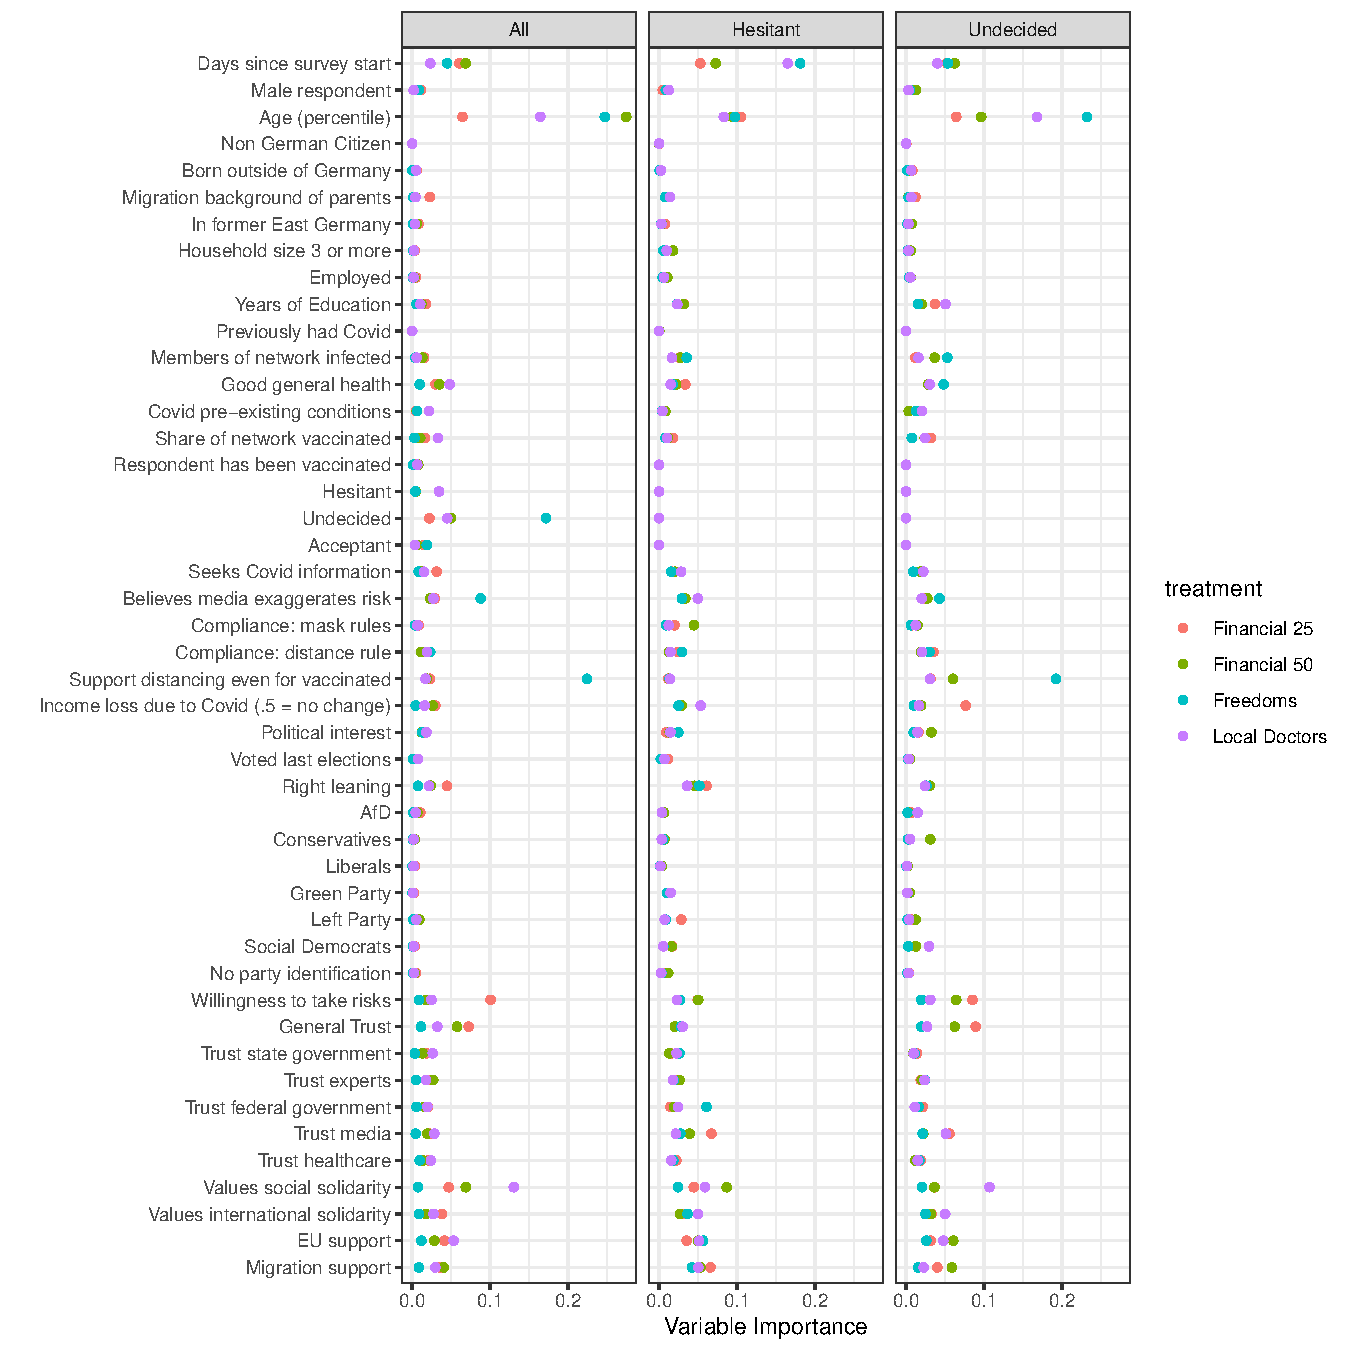
\includegraphics[width=1\linewidth]{figures/figure_3.pdf}
	\caption{\textbf{Predictors of heterogeneous effects.}}
\end{figure}



\clearpage

\subsection{Plotting heterogeneous effects by age}

%%%%%%%%%%%%%
\begin{figure}[h!]
	\centering
	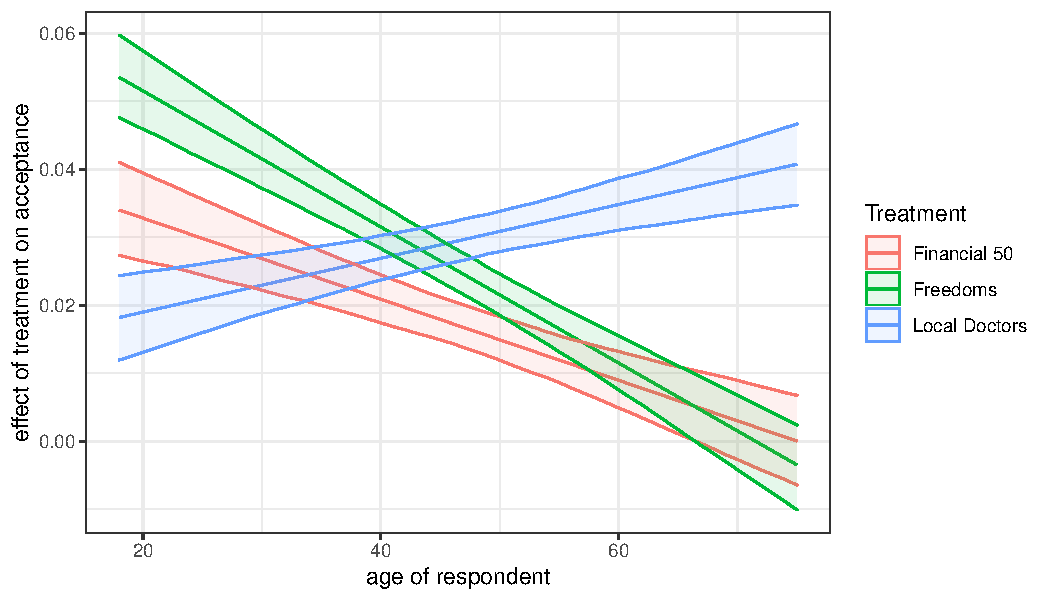
\includegraphics[width=1\linewidth]{figures/figure_12.pdf}
	\caption{\textbf{Treatments effects depend on the age of respondents.}}
\end{figure}



\clearpage


\end{document}




















